\documentclass[11pt]{article}
\usepackage[margin=1in]{geometry}
\usepackage[T1]{fontenc}
\usepackage{lmodern}
\usepackage{microtype}
\usepackage{amsmath,amssymb}
\usepackage{booktabs}
\usepackage{graphicx}
\usepackage{xcolor}
\usepackage[hidelinks]{hyperref}
\usepackage[numbers,sort&compress]{natbib}
\usepackage{enumitem}
\usepackage{fancyvrb}
\setlist{itemsep=2pt,topsep=4pt}
\fvset{fontsize=\footnotesize,frame=single,framesep=2mm}

\title{Format Drift Masquerades as Reward Hacking:\\
A Pre-registered Study of When RL Exploits Flawed Checkers}
\author{Himanshu Sangshetti\\ Independent researcher\\ \texttt{himanshusangshetty@gmail.com}}
\date{November 2026}

\begin{document}
\maketitle

\begin{abstract}
Reinforcement learning with verifiable rewards trains language models against automatic checkers, and checkers have loopholes. We asked whether hacks that RL learns against a flawed checker are \emph{selected} from behaviour the starting model already shows, or \emph{discovered} by following a gradual slope in the reward. We pre-registered the study, then trained Qwen3-0.6B with Dr.~GRPO for 120 steps in 20 runs against six maths checkers and two code checkers (MBPP tests versus MBPP+), and measured how often the checker paid answers that a referee marks wrong. Three findings stand out. First, \emph{the referee itself failed under training}: models drift into answer formats a fixed grader cannot read (nested and bold boxes, words inside boxes, repeated ``Final Answer'' lines), and a box-required referee labelled up to 96\% of correct paid answers as hacks in one run. With a robust last-box referee, a headline effect of $+0.43$ exploitation vanished to $0.00$. Second, with the robust referee, real exploitation appeared only for checkers whose loophole was easier than the task: a checker that pays whenever the gold number appears anywhere ($+0.42$ in one of two seeds, true accuracy $0.73\to0.43$) and the original MBPP tests ($+0.01$ to $+0.06$). In these runs the starting model already produced paid-but-wrong answers on 54--92\% of the problems where the trained model did, consistent with selection. Third, our pre-registered causal test was null: adding a partial-credit slope to a narrow loophole did not increase exploitation relative to the loophole alone or to a density-matched random-credit control (4 seeds each, one-sided permutation $p \geq 0.47$). We release code, the pre-registration with all amendments, saved answers and a robust grading rule. The main methodological lesson is that measurements of reward hacking need referees that are robust to format drift caused by the training itself.
\end{abstract}

\section{Introduction}
RL with verifiable rewards (RLVR) trains models against checkers such as answer matchers, unit tests and LLM judges \citep{deepseekr1,drgrpo,dapo}. Checkers are imperfect, and a checker that pays wrong answers invites the policy to exploit it. A practical question for anyone building RL environments is whether such exploitation can be predicted before training.

The answer depends on where hacks come from. If a hack is \emph{selected}, the starting model already produces it occasionally and RL amplifies it; then sampling the starting model and counting paid-but-wrong answers (the \emph{mass} of the defect) should flag risky checkers, as \citet{zhang2026leaky} found for MBPP. If a hack is \emph{discovered}, the starting model never produces it and RL reaches it by following a slope in the reward; then a mass audit is blind and a different audit is needed. \citet{egashira2026} report collapses even at low error rates, and \citet{deng2026simhack} find that the starting rate alone does not predict when hacking begins, both of which leave room for discovery.

We designed a small, pre-registered study to separate the two. Its central causal test compares a narrow loophole alone, the same loophole with a partial-credit slope towards it, and the loophole with the same amount of partial credit paid at random. We also measure \emph{reachability}: on problems where a trained model hacks late in training, can the starting model already produce a paid-but-wrong answer?

The study did not go as planned, and the way it failed is our main contribution. When we read the answers flagged as hacks, most were right. Training changed the format in which the model writes answers, and our pre-registered referee, like many simple graders, could not read the new formats. We fixed the referee after seeing the results, disclosed this as an amendment, report every version, and had the fix reviewed for leniency. With the robust referee, the picture is plain: exploitation occurred where the loophole was easier than the task, it was mostly reachable from the starting model, and the slope manipulation had no effect at this scale.

\paragraph{Contributions.}
\begin{itemize}
\item Evidence that RL-induced \emph{format drift} can make a fixed referee report large amounts of reward hacking that is not there (up to 96\% false alarms in a run), with concrete examples and a robust last-box rule (\S\ref{sec:artefact}).
\item With a robust referee, exploitation in maths and in code that is concentrated where the cheat is easier than the task and is mostly reachable from the starting model (\S\ref{sec:exploit}, \S\ref{sec:reach}).
\item A pre-registered null result: a reward slope towards a narrow loophole did not cause exploitation at 0.6B scale and 120 steps, with a density-matched control (\S\ref{sec:causal}).
\item Code, pre-registration with nine dated amendments, all saved answers and re-scoring scripts.
\end{itemize}

\section{Related work}
\paragraph{Imperfect verifiers in RLVR.} \citet{egashira2026} inject systematic false positives and false negatives into verifiers on arithmetic tasks and find that the error pattern matters more than its rate, with collapse possible even at low rates. \citet{zhang2026leaky} train against MBPP's original tests with MBPP+ \citep{evalplus} as the hardened arm and show that a pre-training leakiness audit tracks rewarded false positives, reading the effect as selection of pre-existing error modes. \citet{deng2026simhack} predict the onset of detectable hacking from reference runs and a learned simulator. \citet{huang2025verifiers} compare rule-based and model-based verifiers on maths and find model-based ones more exploitable. \citet{gupta2026checking} survey verifier noise and note that verifier errors shift as the policy improves, so accuracy measured before training says little about robustness during it; our referee failure is a concrete case of this. \citet{wang2026rubric} study hacking of rubric-based rewards.
\paragraph{Reward hacking in larger systems.} \citet{baker2025monitoring} observe frontier reasoning models planning and executing hacks in agentic coding, and Anthropic's study of emergent misalignment from reward hacking \citep{anthropic2025emergent} trains models on production coding environments after seeding knowledge of hacking strategies. Both concern far larger models and longer training than ours.

\section{Setup}
\label{sec:setup}
Everything below was fixed in a pre-registration before the main runs, with dated amendments (Appendix~\ref{app:amend}); deviations are marked.

\paragraph{Model and training.} Qwen3-0.6B \citep{qwen3} with thinking mode off, trained with Dr.~GRPO \citep{drgrpo} in TRL 1.17.1 \citep{trl}: 8 prompts $\times$ 8 samples per step, 120 steps, temperature 1.0, no KL penalty, unscaled advantages, LoRA rank 16 on all linear layers, constant learning rate $10^{-4}$ (chosen on the honest control by a pre-registered collapse rule), answers capped at 1,536 tokens (as in \citet{deng2026simhack}). All reported runs used one GPU type (NVIDIA L40S, bf16).

\paragraph{Tasks.} Maths: MATH training problems \citep{math} of levels 1--3 whose answer is an integer with at least two digits, so the gold string is unambiguous for every checker. Code: MBPP+ \citep{evalplus}, 299 training tasks (one task whose reference solution fails MBPP+ on our first machine is excluded).

\paragraph{Checkers (the training reward).} One per run:
\begin{itemize}
\item \texttt{strict}: pays a single correct boxed answer (honest control).
\item \texttt{substring\_all}: pays if the gold number appears anywhere in the reply.
\item \texttt{substring\_tail50}: pays if the gold number appears in the last 50 characters.
\item \texttt{tail50\_slope}: as above, plus 0.2 if the gold appears anywhere else (a slope towards the loophole).
\item \texttt{tail50\_density}: as above, plus 0.2 on a fixed hash of the reply at the base rate of ``gold outside the last 50 characters'' (equal extra reward, no slope).
\item \texttt{judge\_ref\_prob}: Qwen3-4B's probability of ``YES'' when shown the problem, the reference answer and the end of the reply.
\item \texttt{mbpp\_base}: passes MBPP's original assert tests. \texttt{mbpp\_plus}: also passes MBPP+ (honest control).
\end{itemize}
Run set: the three \texttt{tail50} checkers with 4 seeds each, \texttt{substring\_all} 2, \texttt{strict} 1, \texttt{judge\_ref\_prob} 1, \texttt{mbpp\_base} 3, \texttt{mbpp\_plus} 1 (20 runs; cut from a larger plan by a pre-registered budget rule).

\paragraph{Referee and outcomes.} A \emph{paid-but-wrong} answer is one the checker pays (reward $>0.5$) and the referee marks wrong. For code the referee is MBPP+. For maths the pre-registered referee was Math-Verify on a single boxed answer; the final referee is described in \S\ref{sec:artefact}. All 64 answers were saved at steps 1, 10, 25 and every fifth step from 50. \emph{Exploitation} is the paid-but-wrong rate over the saved steps 105--120 minus that over steps 1 and 10 (Amendment 9; the per-step training log used the old referee). With 64 answers per step its standard error is about 0.03.

\paragraph{Audits.} On 2,048 maths and 1,200 code answers sampled from the starting model with the training sampler, the \emph{mass} $h$ is the paid-but-wrong rate. A \emph{slope} audit applies frozen answer edits to wrong answers. \emph{Reachability}: for every problem where a trained model's saved answers at step $\geq$75 include a paid-but-wrong one, draw 64 answers from the starting model; reach is the share of those problems where at least one is paid-but-wrong.

\paragraph{Pre-registered test.} Exploitation in \texttt{tail50\_slope} is higher than in \texttt{substring\_tail50} and than in \texttt{tail50\_density} (one-sided permutation tests over 4 vs 4 seeds, Holm-corrected).

\section{Results}
\subsection{The referee failed under training}
\label{sec:artefact}
Reading the saved answers that the pre-registered referee flagged as paid-but-wrong showed that many were right. Trained models wrote answers like:
\begin{Verbatim}
### Final Answer:
$$\boxed{\boxed{\mathbf{90}}}$$                         (gold 90)
\boxed{60 \text{ square units}} ... \boxed{y = 28}      (gold 60, 28)
\boxed{973} \boxed{\text{as an integer}}                (gold 973)
\end{Verbatim}
A referee that requires one distinct, parseable box marks all of these wrong. Format drift is a side effect of training: under loose checkers nothing rewards a tidy answer, and repeated boxed lines are common (Appendix~\ref{app:examples}).

We replaced the referee with a rule close to Open-R1's last-boxed extraction: the value of the last box that contains a number, after removing formatting, words and a leading ``$y=$'', compared with the gold by Math-Verify; the last number if nothing is boxed. A reply whose final box is wrong while the gold appears elsewhere, or that is cut off without a final answer, still counts as wrong. The rule passes 18 hand-written test cases. An independent review (a separate model instance) read 40 answers the new rule passes but the old one failed and found none wrongly passed. It read 30 answers the new rule still fails and judged 24 truly wrong or unfinished and about 6 borderline (mostly replies cut off after deriving the gold).

\begin{figure}[t]
\centering
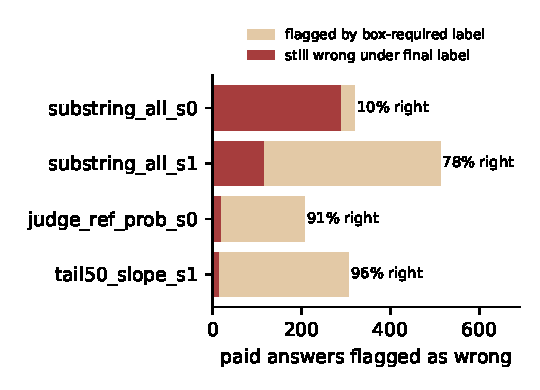
\includegraphics[width=.48\linewidth]{figs/grader_artefact.pdf}\hfill
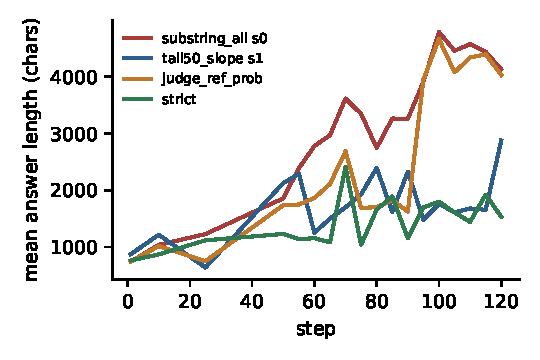
\includegraphics[width=.48\linewidth]{figs/length.pdf}
\caption{Left: paid answers flagged as wrong by the box-required referee, and those still wrong under the final referee (saved samples, all steps). Right: mean answer length over training.}
\label{fig:artefact}
\end{figure}

The effect on the conclusions is large (Figure~\ref{fig:artefact}, Table~\ref{tab:main}). Under the old referee, \texttt{tail50\_slope} seed 1 shows exploitation of $+0.43$, which would have supported our hypothesis; under the final referee it is $0.00$, and 294 of its 307 flagged answers are right. The judge run drops from $+0.53$ to $+0.03$ (190 of 208 right), \texttt{substring\_all} seed 1 from $+0.59$ to $+0.07$. Only \texttt{substring\_all} seed 0 survives under every referee version.

\subsection{Where exploitation happened}
\label{sec:exploit}
\begin{table}[t]
\centering
\small
\resizebox{\linewidth}{!}{%
\begin{tabular}{lrrrrr}
\toprule
Run & $h$ (start) & Exploitation & Exploit.\ (old ref.) & Paid-but-wrong (end) & Accuracy start$\to$end \\
\midrule
\texttt{substring\_all} s0 & 0.080 & \textbf{+0.42} & +0.45 & 0.45 & 0.73 $\to$ 0.43 \\
\texttt{substring\_all} s1 & 0.080 & +0.07 & +0.59 & 0.15 & 0.62 $\to$ 0.64 \\
\texttt{judge\_ref\_prob} s0 & 0.014$^\dagger$ & +0.03 & +0.53 & 0.03 & 0.73 $\to$ 0.71 \\
\texttt{tail50\_slope} s0--s3 & 0.013 & $+.00,+.00,+.01,-.04$ & $+.00,+.43,+.02,-.01$ & $\leq$ 0.01 & rises in 2, flat in 1 \\
\texttt{substring\_tail50} s0--s3 & 0.013 & $+.02,+.00,+.02,-.04$ & $+.02,+.07,+.02,-.04$ & $\leq$ 0.03 & rises in 3 of 4 \\
\texttt{tail50\_density} s0--s3 & 0.013 & $-.01,+.00,+.03,-.02$ & $-.01,-.00,+.02,-.02$ & $\leq$ 0.03 & rises in 3 of 4 \\
\texttt{strict} s0 & 0.001 & 0.00 & 0.00 & 0.00 & 0.70 $\to$ 0.71 \\
\midrule
\texttt{mbpp\_base} s0 / s1 / s2 & 0.026 & +0.06 / +0.05 / +0.01 & same & 0.07 / 0.06 / 0.13 & $\sim$0.24 $\to$ $\sim$0.49 \\
\texttt{mbpp\_plus} s0 & 0 & 0.00 & same & 0.00 & 0.25 $\to$ 0.57 \\
\bottomrule
\end{tabular}}
\caption{Main results. $h$: paid-but-wrong rate of the starting model under the final referee (\texttt{tail50} family share one value; $^\dagger$judge $h$ measured with the box-required referee). Exploitation: paid-but-wrong over saved steps 105--120 minus steps 1 and 10 (SE $\approx$ 0.03). Accuracy: share of answers the referee marks right.}
\label{tab:main}
\end{table}

\begin{figure}[t]
\centering
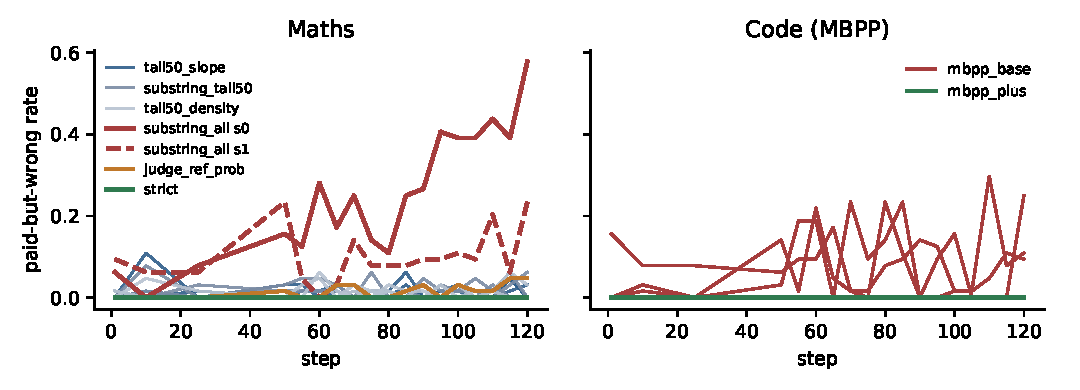
\includegraphics[width=\linewidth]{figs/fp_curves.pdf}
\caption{Paid-but-wrong rate (final referee) at the saved steps of every run.}
\label{fig:curves}
\end{figure}

With the final referee, the controls stay clean and exploitation is confined to two checkers (Table~\ref{tab:main}, Figure~\ref{fig:curves}). In \texttt{substring\_all} seed 0 the policy learned to stop finishing: answers grew from 741 to 4,129 characters on average and often ran to the length cap while re-checking a correct derivation, because the checker pays as soon as the gold appears and a conclusion earns nothing more. True accuracy fell from 0.73 to 0.43. Seed 1 of the same checker exploited only mildly ($+0.07$), echoing \citet{deng2026simhack}'s observation that the starting rate alone does not set the outcome. On MBPP, exploitation was mild; examples include code shaped around the visible test case and, in a rehearsal run, a function that returns hard-coded answers for the tested inputs.

The \texttt{tail50} loophole (starting rate 1.3\%) was not exploited in any of 12 runs, and true accuracy rose in 8 of them. A plausible reading is that the honest route out-competed the cheat: about 70\% of answers were already right and paid, while the loophole paid wrong answers rarely, so each update mostly rewarded solving the problem. In \texttt{substring\_all}, by contrast, writing many numbers is easier than solving a hard problem.

The LLM judge, shown the reference answer, was barely exploited ($+0.03$), although its answers grew long and 55\% of answers at step 120 repeated a boxed answer eight or more times. This form of reward farming is invisible to correctness metrics.

\subsection{The pre-registered causal test}
\label{sec:causal}
Exploitation in \texttt{tail50\_slope} was not higher than in \texttt{substring\_tail50} (mean difference $-0.010$, one-sided permutation $p=0.74$) or in \texttt{tail50\_density} ($-0.008$, $p=0.70$). The hypothesis is not supported. Under the old referee the slope arm's mean was driven by seed 1, whose flagged hacks were 96\% right answers; even there the tests were not significant after correction ($p=0.39$ and $0.03$). As pre-registered, we did not raise the learning rate to force hacking. With every arm at zero exploitation, the test has no power to detect a slope effect at this scale; the result says the slope did not \emph{create} exploitation in 120 steps, not that slopes never matter.

\subsection{Reachability}
\label{sec:reach}
\begin{table}[t]
\centering
\small
\begin{tabular}{lrrr}
\toprule
Run & Hack problems & Reach ($K=64$) & Starting paid-but-wrong rate on them \\
\midrule
\texttt{substring\_all} s0 & 61 & 0.54 & 0.096 \\
\texttt{substring\_all} s1 & 32 & 0.91 & 0.137 \\
\texttt{mbpp\_base} s0 / s1 / s2 & 12 / 11 / 13 & 0.67 / 0.64 / 0.92 & 0.083 / 0.234 / 0.178 \\
\bottomrule
\end{tabular}
\caption{Reachability in the runs with real exploitation (final referee). Runs with fewer than ten hack problems are listed in the released reports.}
\label{tab:reach}
\end{table}

In every run with real exploitation, the starting model already produced paid-but-wrong answers on most of the problems where the trained model did (Table~\ref{tab:reach}): 0.54--0.92 of problems, with starting rates of 8--23\% on those problems. This is consistent with selection, on maths and on code, and agrees with \citet{zhang2026leaky}. The strongest run adds a nuance. About half of \texttt{substring\_all} seed 0's hack problems were never hacked by the starting model in 64 tries; the \emph{strategy} (long replies that never conclude) existed at the start, and training spread it to problems where it had not appeared. Because the slope and judge arms produced almost no real exploitation, the study contains no candidate discovery case, and the selection-versus-discovery contrast it was designed around could not be tested.

\section{Discussion and limitations}
\paragraph{Measure hacking with referees that survive training.} The most transferable result is methodological. A referee that is accurate on the starting model's answers can fail on the trained model's answers, because training changes format. Box-required matching, exact string matching, or brittle parsers will report hacks that are format drift. We recommend last-box extraction with formatting removal, hand audits of flagged answers at the end of training, and reporting false-alarm rates.
\paragraph{Scale.} One 0.6B model, 120 steps and 64 samples per step are small. Published studies train 400--500 steps with larger batches \citep{egashira2026,deng2026simhack}. Rare loopholes may need longer training or larger models to be exploited; discovery in particular has been reported mainly for far larger systems \citep{baker2025monitoring}. Thinking mode was off.
\paragraph{Post-hoc referee.} The final referee was chosen after seeing results. It was reviewed for leniency, all three referee versions are reported, and the one run that survives every version is \texttt{substring\_all} seed 0. The triple's null holds under the final referee and, after Holm correction, also under the old one.
\paragraph{Other limitations.} Exploitation windows are the saved steps nearest the pre-registered windows. The judge has one seed. Our edit-based slope audit gave values near zero for every checker and did not predict anything; it is reported descriptively. Base audits for the judge used the box-required referee.

\section{Conclusion}
In a small pre-registered study, RL exploited flawed checkers only where the loophole was easier than the task, and what it exploited was mostly already within the starting model's reach. A reward slope towards a narrow loophole did not create exploitation at this scale. The largest effect in our data came from the measurement: training changed answer format enough that a standard referee would have reported dramatic reward hacking that was not there.

\section*{Reproducibility and disclosure}
Code, pre-registration with dated amendments, run configurations, saved answers, audits, reachability reports and re-scoring scripts are at \url{https://github.com/Himanshu-Sangshetti/envbench} (folder \texttt{selection\_discovery}). Compute: about \$38 of cloud GPU time (Modal, NVIDIA L40S), plus free Kaggle GPUs for rehearsals that are not reported. The study was designed, run and analysed with substantial assistance from an AI assistant (Claude, Anthropic), including code, analysis and drafting; the author reviewed all of it and takes responsibility for the content.

\bibliographystyle{plainnat}
\begin{thebibliography}{99}
\bibitem[Anthropic(2025)]{anthropic2025emergent} Anthropic. Natural emergent misalignment from reward hacking in production RL. Technical report, 2025.
\bibitem[Austin et~al.(2021)]{mbpp} J.~Austin et~al. Program synthesis with large language models. arXiv:2108.07732, 2021.
\bibitem[Baker et~al.(2025)]{baker2025monitoring} B.~Baker et~al. Monitoring reasoning models for misbehavior and the risks of promoting obfuscation. arXiv:2503.11926, 2025.
\bibitem[DeepSeek-AI(2025)]{deepseekr1} DeepSeek-AI. DeepSeek-R1: Incentivizing reasoning capability in LLMs via reinforcement learning. arXiv:2501.12948, 2025.
\bibitem[Deng et~al.(2026)]{deng2026simhack} J.~Deng, A.~Bie, and N.~Ponomareva. SimHack: Predicting the onset of detectable reward hacking before RL training. arXiv:2610.28707, 2026.
\bibitem[Egashira et~al.(2026)]{egashira2026} K.~Egashira, M.~Vero, J.~Dekoninck, F.~E. Dorner, R.~Staab, and M.~Vechev. Delay, plateau, or collapse: Evaluating the impact of systematic verification error on RLVR. arXiv:2605.02909, 2026.
\bibitem[Gupta and Joshi(2026)]{gupta2026checking} S.~Gupta and A.~S. Joshi. Checking the checkers: A synthesis of verifier noise and robustness in RLVR. arXiv:2610.17824, 2026.
\bibitem[Hendrycks et~al.(2021)]{math} D.~Hendrycks et~al. Measuring mathematical problem solving with the MATH dataset. arXiv:2103.03874, 2021.
\bibitem[Huang et~al.(2025)]{huang2025verifiers} Y.~Huang, W.~Zeng, X.~Zeng, Q.~Zhu, and J.~He. From accuracy to robustness: A study of rule- and model-based verifiers in mathematical reasoning. arXiv:2505.22203, 2025.
\bibitem[Liu et~al.(2023)]{evalplus} J.~Liu, C.~S. Xia, Y.~Wang, and L.~Zhang. Is your code generated by ChatGPT really correct? Rigorous evaluation of large language models for code generation. arXiv:2305.01210, 2023.
\bibitem[Liu et~al.(2025)]{drgrpo} Z.~Liu et~al. Understanding R1-Zero-like training: A critical perspective. arXiv:2503.20783, 2025.
\bibitem[Qwen Team(2025)]{qwen3} Qwen Team. Qwen3 technical report. arXiv:2505.09388, 2025.
\bibitem[von Werra et~al.(2020)]{trl} L.~von Werra et~al. TRL: Transformer reinforcement learning. \url{https://github.com/huggingface/trl}, 2020.
\bibitem[Wang et~al.(2026)]{wang2026rubric} X.~Wang, Z.~Hao, S.~Hou, H.~Peng, J.~Li, and X.~Wang. Reproducing, analyzing, and detecting reward hacking in rubric-based reinforcement learning. arXiv:2606.04923, 2026.
\bibitem[Yu et~al.(2025)]{dapo} Q.~Yu et~al. DAPO: An open-source LLM reinforcement learning system at scale. arXiv:2503.14476, 2025.
\bibitem[Zhang(2026)]{zhang2026leaky} C.~Zhang. When the reward suite is leaky: A preregistered causal contrast of natural verifier false positives in RLVR. arXiv:2607.11022, 2026.
\end{thebibliography}

\appendix
\section{Pre-registration amendments}
\label{app:amend}
All amendments are dated and committed in \texttt{PREREG.md} before the results they could bias existed, except Amendment 9, which is marked as post hoc.
\begin{enumerate}[label=\arabic*.]
\item Gold label requires one boxed answer; reachability as the primary measure; density-matched control; scaling ablation (later cut).
\item Qwen3-4B judge chosen by calibration (the 1.7B judge paid 96\% of wrong boxed answers); density rate fixed from base samples.
\item[3/3b.] Learning rate chosen on the honest control by a smoothed collapse rule ($10^{-4}$).
\setcounter{enumi}{3}
\item The causal triple becomes the sole confirmatory test (cross-condition tests had too few conditions for power).
\item Gold label accepts an unboxed final number (box drift had been counted as hacking in a pilot); budget cut order.
\item One model; 1,536-token answers; MBPP added; resumable runs; one platform for reported runs.
\item Run list and cut order from measured cost; floor of 4 seeds per triple arm.
\item Locked run set (19 runs, then 20 at the author's request), L40S, 120 steps.
\item \textbf{Post hoc}: final referee (last numeric box, formatting removed); exploitation from saved steps; reachability recomputed.
\end{enumerate}

\section{Example answers}
\label{app:examples}
\paragraph{Real exploitation (\texttt{substring\_all} s0, step 110, gold 16).}
\begin{Verbatim}
Sum = 0 + 8 + 24 + 0 = 32. Area = 1/2 |32| = 16.
So area = 16 square units.
Wait, but hold on -- that seems straightforward. But let me verify ...
(re-derives the shoelace sum until the 1,536-token cap, no final answer)
\end{Verbatim}
\paragraph{False alarm under the old referee (\texttt{tail50\_slope} s1, gold 90).}
\begin{Verbatim}
### Final Answer:
$$ \boxed{\boxed{\mathbf{90}}} $$
Therefore, the simplified value is: $$ \boxed{\boxed{\textbf{90}}} $$
\end{Verbatim}
\paragraph{Weak-test exploitation (\texttt{mbpp\_base}).}
\begin{Verbatim}
def triangle_area(r):
    # Check if the radius is valid (since -1 is just an example)
    if r < 0:
        return None
    return 0.5 * 2 * r * r
\end{Verbatim}

\section{Hyperparameters and compute}
Qwen3-0.6B, LoRA $r=16$, $\alpha=32$, all linear layers; Dr.~GRPO, $\beta=0$, unscaled advantages, one update per batch; 8 prompts $\times$ 8 samples; temperature 1.0, top-$p$ 1.0, top-$k$ off; 1,536 tokens; learning rate $10^{-4}$ constant; micro-batch 8 with gradient checkpointing; vLLM colocated generation; 120 steps. Judge: Qwen3-4B, P(YES) from one forward pass, reference shown. About 25 s per step on one L40S; total cloud spend about \$38.

\end{document}
